\section{Results}

In this section, we consider data for each research questions in more detail.

\subsection{{\bf RQ1}: Comparing news and Twitter } 
\begin{figure}[t]
	\centering
	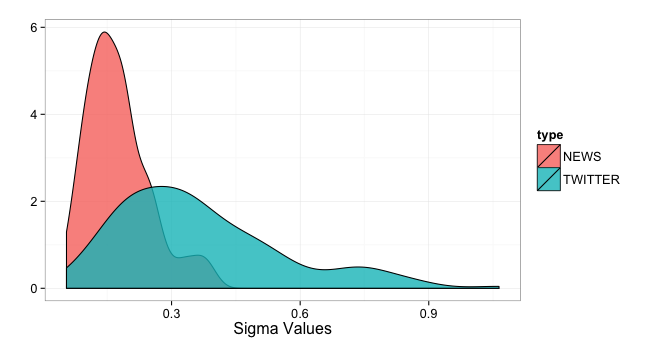
\includegraphics[width=.5\textwidth]{imgs/diff_sigma}
	\caption{Distribution of Sigmas}
	\label{fig:sig}
\end{figure}

While a host of comparisons could be made between the news and Twitter data we study, we restricted ourselves here to a subset of questions of particular interest. First, we are interested in the level of variance over time in discussions of particular themes in particular countries on Twitter as compared to in news.  Conveniently, our statistical model provides us with a parameter, $\sigma^2_{w,r}$ which captures the extent of this variability. Figure~\ref{fig:sig} shows a density plot detailing the distribution of values for $\sigma^2_{w,r}$ for the news and Twitter data.  As is clear, Twitter data is much more variable in the news, both in the average variability across a particular theme/country time series and with respect to the expected value of $\sigma^2_{w,r}$ in general.  This finding shows that news coverage of the Arab Spring was more stable than discussion on Twitter.  Our results correlate with the idea that while the propagation of content is similar in form in both Twitter and news media,  the social elements of Twitter introduce important variability in the diffusion and longevity of discussion \citep{yang_patterns_2011}.  Perhaps more importantly, our findings show that the extent to which a change in thematic focus is ``interesting'' differs when analyzing news versus Twitter data. Researchers using social media data to interpret change in social processes, our data suggests, must be more cautious than those with access to news data.

In addition to levels of variability in the two media, we are also interested in the extent to which news and Twitter data focused on the same topics at the same time.  That is, we are interested in the extent to which the time series of $\eta_{w,r,t}$ values for Twitter and news are correlated for a particular theme/country combination.  Importantly, this correlation cannot be measured directly with our $\eta_{w,r,t}$ - baked into our model is the assumption of autocorrelation with a one-month lag (Equation~\ref{eq:eta_eq}), which will lead to spuriously high correlation values.  To infer correlations between news and Twitter data, we therefore must remove the autocorrelation by subtracting the prior month's value from each activation score.  More specifically, for a given country $r$ and category $w$, we construct a vector of observations $\eta_{w,r,t}-\eta_{w,r,t-1} \quad \forall \, t > 1$ for both Twitter and news data. These vectors are, via the assumptions of our model, void of autocorrelation and can therefore be compared directly using, for example, a simple Pearson correlation.

The first question is whether or not there is a significant correlation between the news and Twitter across all countries and themes. Importantly, we would expect this correlation to be positive and significant for the non-stopword data, and to be close to zero for our stopword themes. Using the bootstrap procedure  with 10000 iterations, we construct 99\% confidence intervals using a pivot interval \citep{wasserman_all_2003} on the Pearson correlation between news and Twitter data. That is, we determine the extent to which the changes in activation from the previous month in Twitter data are linearly correlated with changes from the previous month in news data, taking as input all observations across all countries.  We perform this analysis twice, once for the non-noise (non-Stopword) themes and once for the noise-only themes.


The correlation for the non-noise data is .23 [.17,.28], indicating a moderate but significant correlation between news and Twitter.  There are several reasons for the existence of this correlation. Perhaps most importantly, it is well known that news agencies send tweets about their key stories, and retweets of these stories comprise an important component of discussion on Twitter. Thus news and Twitter should be correlated, as they form a part of a symbiotic media system.  In some sense, it is therefore interesting that the correlation between the two media is not higher.  One obvious reason is that personal, socially-focused discussions do of course occur on Twitter. Additionally, a large volume of tweets are known to be sent by bots on Twitter, many of which are just tweeting nonsense phrases.

The correlation for the noise-only data was .1 [-.001, .19].  Results suggest that correlations between non-noise themes is (significantly) greater than noise themes, and that the noise data was not significantly different from 0 at $\alpha=.01$. However, results do indicate that there may still be some level of correlation in the residual noise in our data between news and Twitter.  This may be due to a variety of factors, perhaps most obviously the fact that we treat each country independently.  While future work may consider means of addressing these biases, we instead choose here only to account for the possible existence of this spurious correlation when considering further results. We now turn to explore which themes had the strongest and weakest correlations between news and Twitter (across all countries). 

\begin{figure}
	\centering
	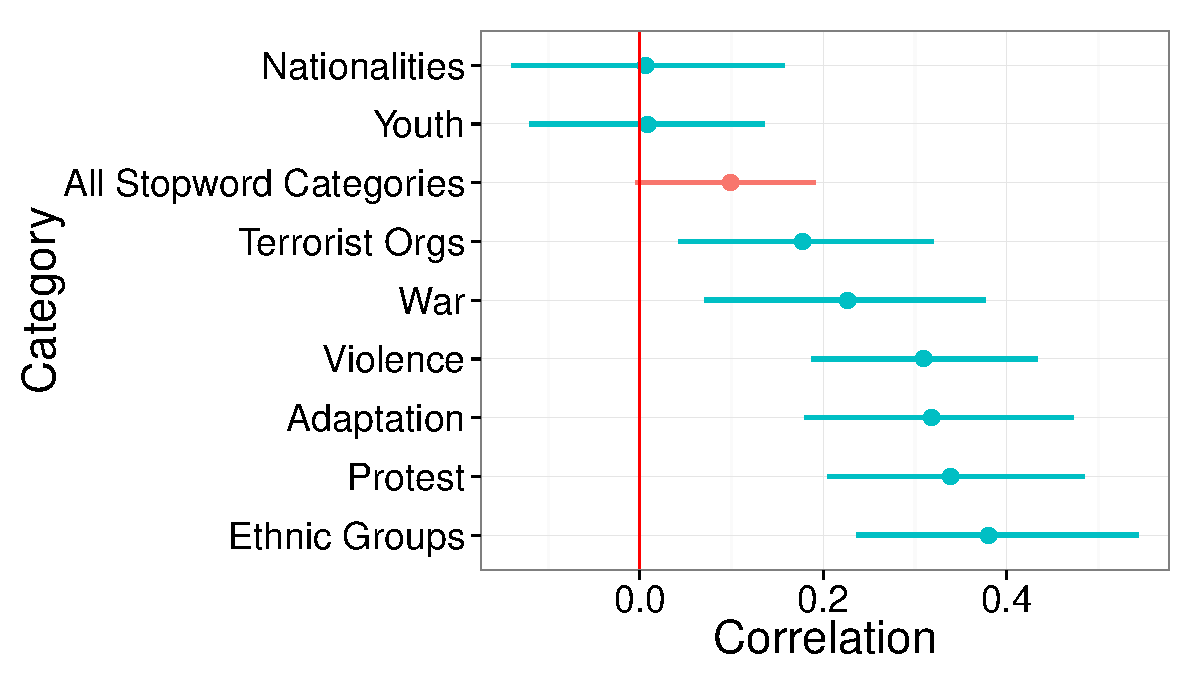
\includegraphics[width=.5\textwidth]{imgs/cat_corr}
	\caption{News/Twitter correlations by category.  Confidence intervals are 99\% bootstrapped CIs calculated with a pivot interval and 10000 iterations}
	\label{fig:cat_corr}
\end{figure}

Figure~\ref{fig:cat_corr} presents the correlations between news and Twitter data for each category, with data aggregated across countries. Additionally, we have aggregated all noise categories into a single category, entitled "All Stopword Categories".  Confidence intervals are constructed in the same way as above, and are shown in the figure via the lines for each category. Mean estimates are shown with a dot.  Figure~\ref{fig:cat_corr} shows that the strongest correlations between news and Twitter occur in reference to general indicators of revolution, specifically, protest and violence. The general level of correlation across these categories supports the idea that news and Twitter discussions specific to the revolution fed off of each other \citep{cottle_media_2011,comunello_will_2012}. Additionally, we can expect that this may be due to the fact that the Tweets by news agencies are focusing in this area. In addition, we observe strong correlations between media in discussions of adaptation and change and to ethnicity. 

On the other hand, in comparison to the Stopword categories,  there is no significant correlation\footnote{at a level of $\alpha=.001$ using the parametric test described in \citep{zou_toward_2007}} for discussions of national identity, youth movements, terrorist organizations and war.  With reference to the ``selecting on the dependent variable'' problem in social media research \citep{tufekci_big_2014}, our findings indicate that scholars focusing too heavily on particular topics may over or under-estimate the correlations between topical focuses of news and Twitter.  Perhaps most interesting is the fact that while discussion of Ethnic, or non-national, identities was highly correlated between the two media, discussion of national identities show little, if any, correlation between media  This difference is important in considering the extent to which news or Twitter data can be used to support the idea of an evolving national identity in contrast to factionalized identities, and suggests that the evolution of a national identity may be a factionated process that is not well monitored by using a single media source. Thus, in future study of \citeapos{goldstone_cross-class_2011} hypotheses on how the proliferation of national identity was important to the success of revolutions, one must consider both news media and Twitter separately in attempting to understand how the existence of a national identity played out in the media landscape surrounding the Arab Spring.   

\begin{figure}
	\centering
	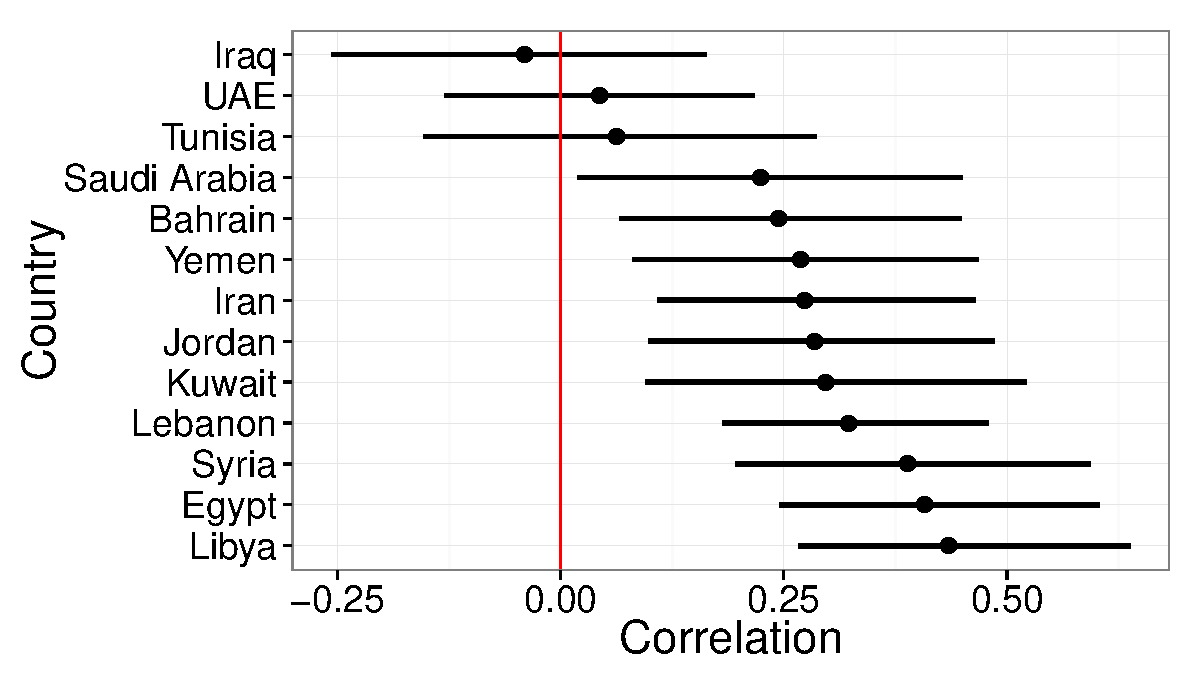
\includegraphics[width=.5\textwidth]{imgs/country_corr}
	\caption{News/Twitter correlations by country}
	\label{fig:corr_country}
\end{figure}

Finally, Figure~\ref{fig:corr_country}  shows correlations between news and Twitter across countries, aggregating across all non-noise themes.  Here, as there is no noise baseline to compare to, we only consider differences from zero in our interpretation.  In light of previous work, the most interesting point to be taken from Figure~\ref{fig:corr_country} is that countries where data has been compared across news and Twitter in the past differ in the ways in which news relates to Twitter. In particular, while there are high levels of correlation between news and Twitter in Libya, Syria and Egypt, no significant correlation exists between these two media in Tunisia.  This implicates the fact that consideration of a single country may also lead to biased conclusions on the relationship between news and Twitter during the Arab Spring. More specifically, it seems that in countries with sustained levels of civil unrest (Syria, Egypt and Libya), news and Twitter are more likely to converge on thematic discussions. In contrast, in countries like Tunisia, where the majority of the civil unrest was short-lived, thematic discussions appear to deviate between the two media. Similarly, correlations in nations where no massive government change occurred show only weak or non-existent correlations between the media.  This may be because in these countries the discussion in the news was on political, economic an global events, but in Twitter it focused on social, cultural and personal events.

\subsection{{\bf RQ2:} Relating to events on the ground}

\begin{table*}[t]
\centering
\begin{tabularx}{\textwidth}{|m{.3cm}| l| l| l| l| m{.7cm}|  X |}
  \hline
 N & Category & Country & Media & Date & +/- Change & Major Event \\ 
  \hline
1 & War & Syria & News & 3/2011 & - & Week of March 15-21 is considered to be the beginning of the Syrian uprising\footnote{\url{http://en.wikipedia.org/wiki/Syrian_Civil_War#Protests_and_armed_insurgency_.28July_.E2.80.93_October_2011.29}} \\   \hline
  2 & Protest & Syria & News & 3/2011 & + &Week of March 15-21 is considered to be the beginning of the Syrian uprising \\   \hline
  3 & Ethnic Groups & UAE & Twitter & 10/2012 & + & EU report condemning human rights climate in UAE \\   \hline
  4 & Protest & Tunisia & Twitter & 8/2012 & + & Tunisian women stage large protests\footnote{\url{http://www.aljazeera.com/indepth/features/2012/08/201281981854620325.html}} \\   \hline
  5 & War & Lebanon & News & 3/2011 &  - & Major rallies throughout the nation on various days\footnote{\url{http://en.wikipedia.org/wiki/2011_Lebanese_protests}}\\   \hline
  6 & Adaptation & Libya & Twitter & 8/2012 & + & First free elections were held in Libya in July, 2012   \\ \hline
  7 & Adaptation & Tunisia & Twitter & 10/2011 &  - & First free election in Tunisia since 1956\footnote{\url{http://en.wikipedia.org/wiki/Tunisian_Constituent_Assembly_election,_2011}} \\   \hline
  8 & Terrorist Orgs & Libya & News & 9/2012& + & Attack on U.S. consulate in Benghazi, Libya \\   \hline 
  9 & Terrorist Orgs & Egypt & Twitter & 11/2012 & + & Major protests in Tahrir Square and the beginning of Parliamentary Elections \\  \hline 
  10 & Adaptation & UAE & Twitter & 10/2012 &  - & EU report condemning human rights climate in UAE  \\ 
   \hline
\end{tabularx}
\caption{The top 10 most surprising changes in activation from the previous month.  The column ``+/- change'' indicates if the change was an increase or decrease in activation.  The column ``Major Events'' gives an explanation of the major events that occurred during that month or the previous month (as change is relative to the previous month), or none if no such event occurred.}
\label{tab:events}
\end{table*}

In this section, we explore the extent to which large, sudden changes in activation rates in particular theme/country pairs were indicative of important real-world changes occurring in the Arab world.  Table~\ref{tab:events} lists the ten most ``surprising'' jumps in terms of change in activation from one month to the next.  We ranked the extent to which events were surprising using absolute change in activation, controlling for the overall level of variance for a particular theme/country pair.  That is, for month $t$ in country $r$ for theme $w$, surprise was calculated as $\frac{|\eta_{w,r,t}-\eta_{w,r,t-1}|}{\sigma^2_{w,r}}$.  Table~\ref{tab:events} also shows whether the change was positive or negative (in the column ``+/- change'') and briefly details the major events we believe led to this change.  

Model output shows that the beginning of the Syrian Civil War had the strongest impact on news media. Discussion of war decreased significantly relative to the previous month, as reporters sought to cover the increasing volume and intensity of protests throughout the country. These events, of course, marked the beginning of a civil war that is still well under way (as of the time of writing), showing the model’s propensity to capture important changes in events via news media. In general, sizeable changes in news media’s topical coverage were relevant to emergent protests. Interestingly, this focus appears to manifest in our model as a decrease in discussion of war as opposed to an increase in the discussion of protest. That is, the shift of news coverage away from war or the possibility of war is as indicative of critical protest events as is discussion of the protests themselves. We will see that this effect is significant in interpreting news discussion with respect to Libya, as we explore in our case study. 

In contrast to news media, the most prominent events that caused observable large shifts on Twitter were elections. In Libya and Tunisia, elections led to differences in discussions of adaptation and change, a sign that these elections may have promoted an influx of hopeful discussion of a new era in these countries. In contrast, in Egypt, elections led to increased discussions on organizations with known connections to terrorism, for example, the Muslim Brotherhood or al-Qaeda. The difference in thematic focus in these different elections is an important implication of the differences regarding sentiments towards the elections in each country, and something of interest to future work In addition to elections, the gender equality protests in Tunisia, staged heavily on social media \citep{yuce_womens_2015}, appear as a signal in the Twitter data but not in the news data.  

Finally, with respect to the Twitter data, two entries relating to the UAE in Table~\ref{tab:events}, both of which are relevant to the publication of a European Union report condemning human rights conditions for certain ethnic groups in the country, show up as events which captured a surprising level of discussion relative to the general level of focus on the themes of ethnic identity and adaptation to change in the UAE. Similarly, in the news data, a surprising level of discussion focuses on the attack of a U.S. consulate in Benghazi, Libya.  These issues were relatively minor with respect to their implications for the Arab Spring, but relatively major with respect to the interest drawn to them by U.S. and U.K. media.  The change in discussion that resulted from these events is thus a reminder that the Western-media centric data utilized for this study presents a possible roadblock in 

